\chapter{Conclusion}\label{chapter:conclusion}

\noindent To validate the first hypothesis, which states that using GraphQL with a shared caching layer and a query reduction mechanism can prevent excessive retrievals and over-queries, a micro-frontend architecture with four \acp{SPA} and eight widgets was designed and implemented. An image showing the dashboard of the micro-frontend prototype is shown in Figure \ref{fig:conclusion:ui-dashboard}.

\ifshowImages
\begin{figure}[H]
  \centering
  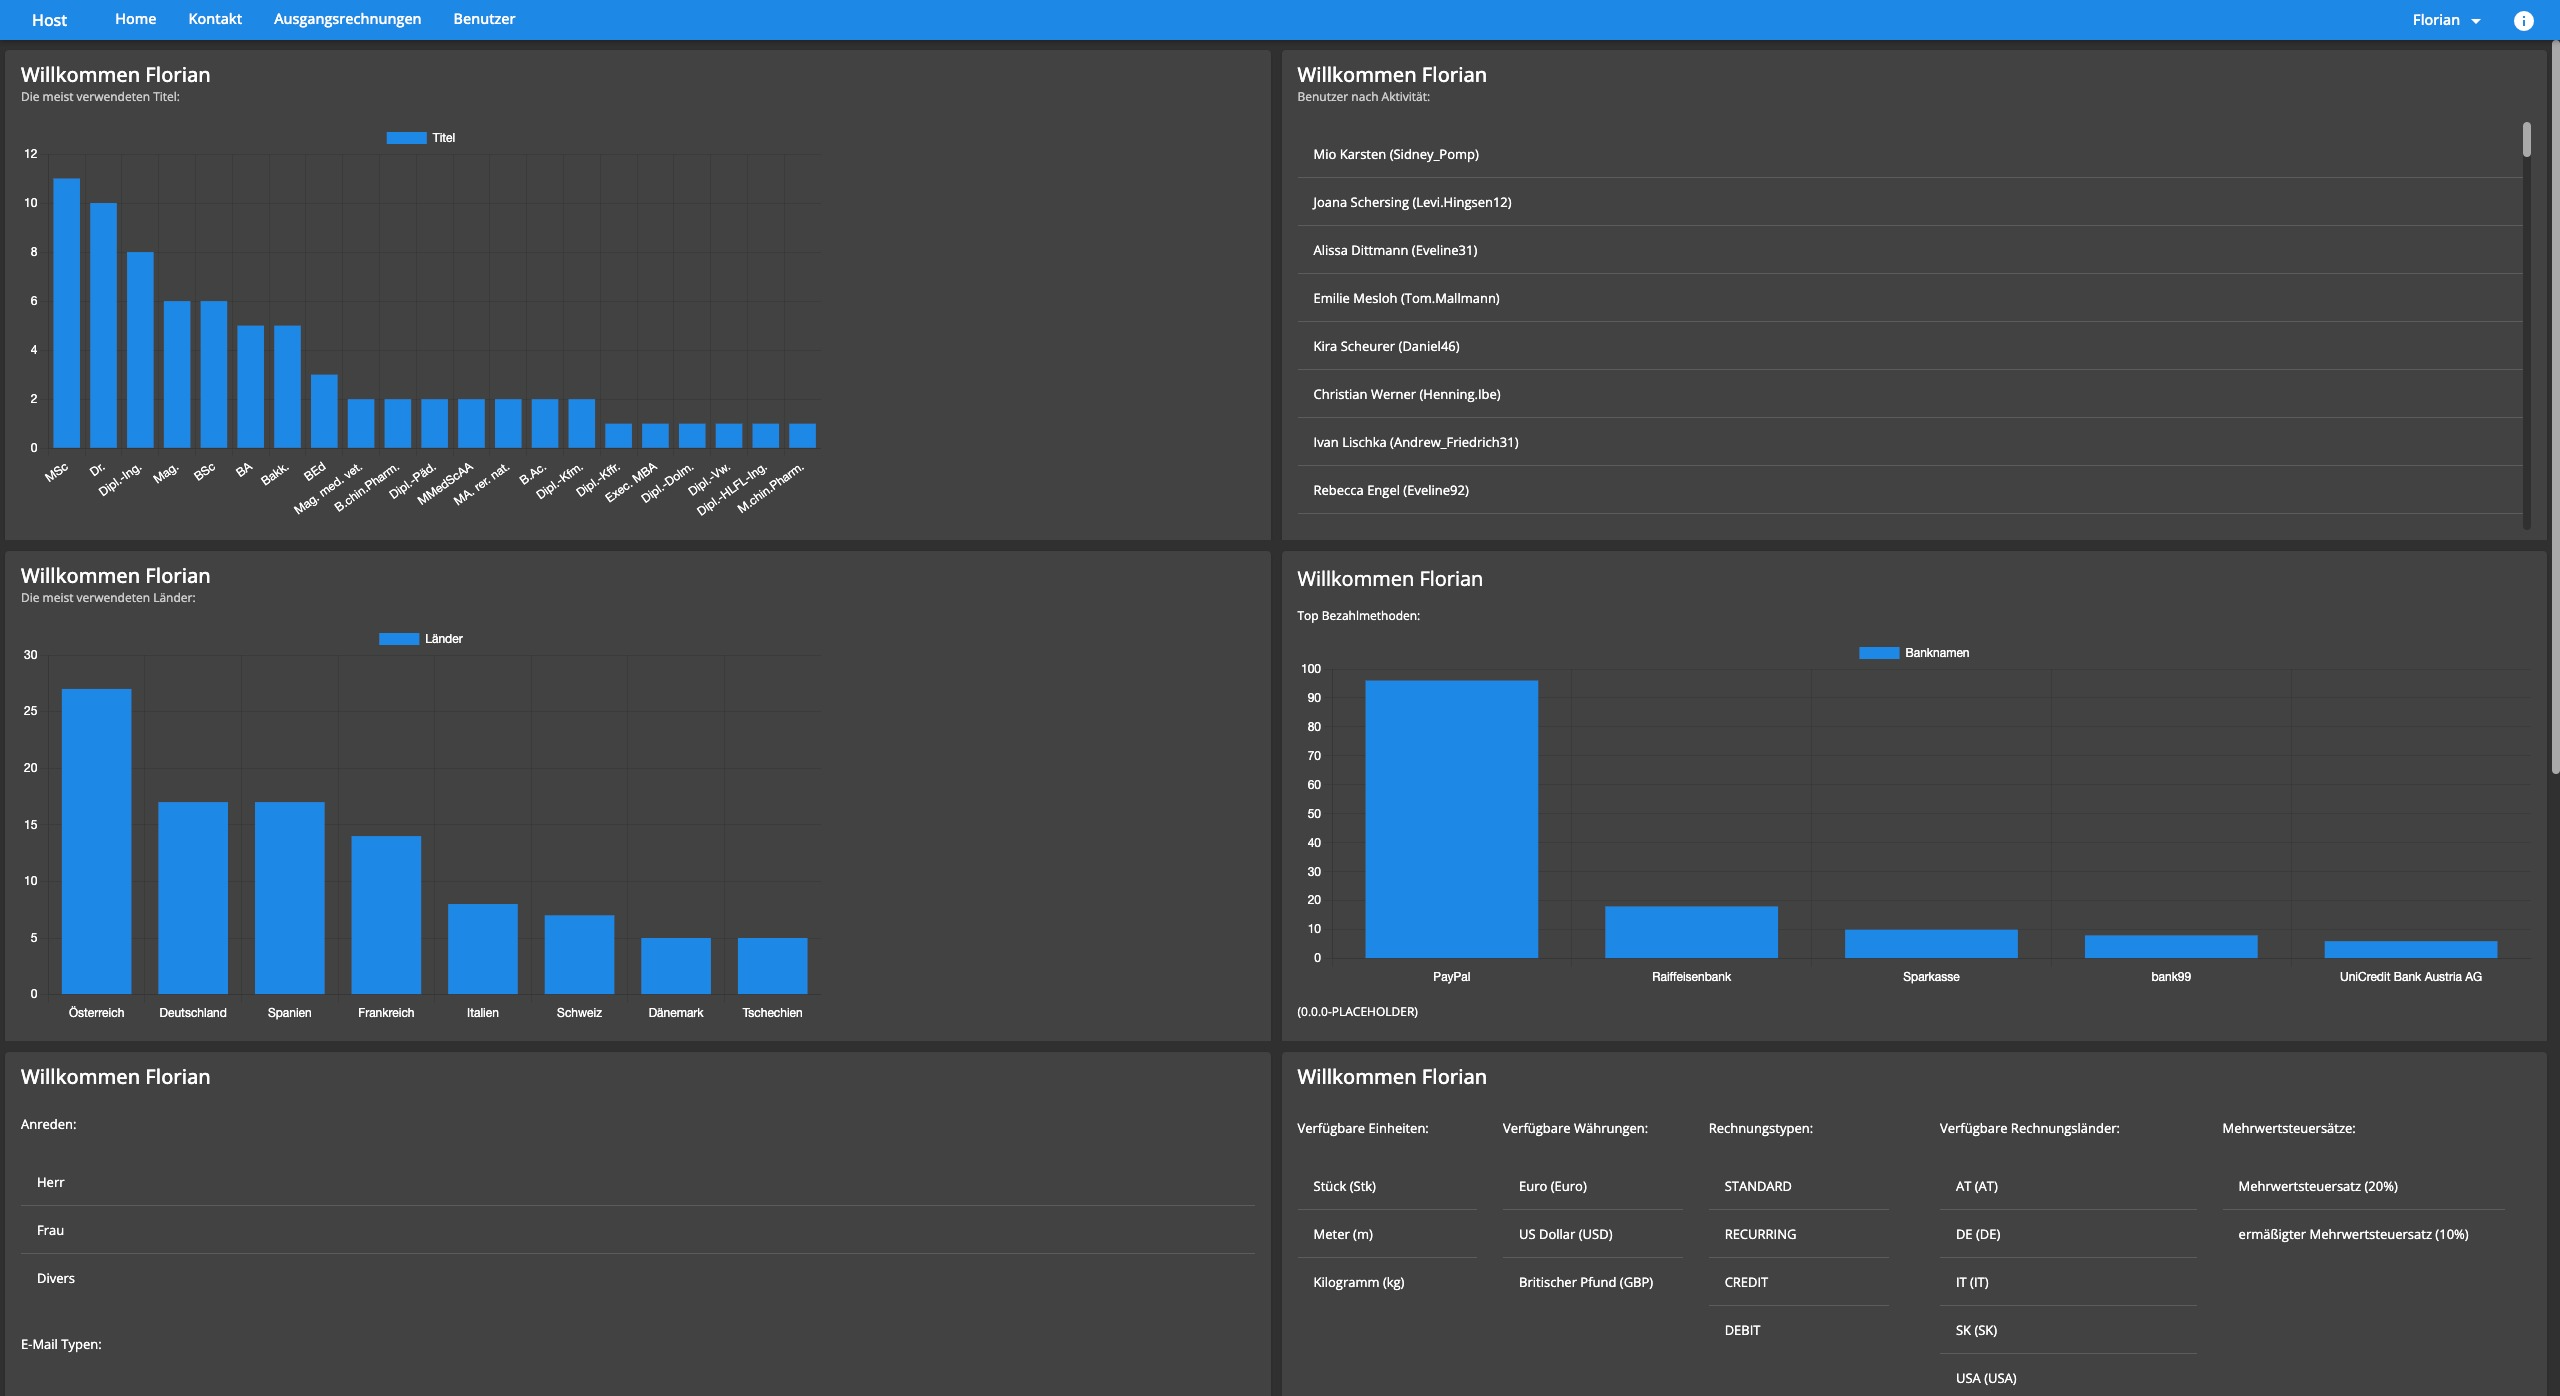
\includegraphics[width=1\linewidth]{images/prototype-screenshots/ui-dashboard.png}
  \caption{The dashboard of the micro-frontend prototype.}\label{fig:conclusion:ui-dashboard}
\end{figure}
\fi

\noindent Before the implementation began, the old legacy system was analyzed to identify potential bounded contexts that could be extracted into separate micro-frontends. The prototype was implemented using mainly Angular and React for a single widget. The micro-frontends were integrated using client-side integration using Webpack's Module Federation. A \ac{BFF} service in the form of a GraphQL \ac{API} was implemented using Apollo Server. This service provides a gateway to the microservice \acp{API} that run inside the company's cluster. The \ac{BFF} takes care of fetching and aggregating the data from multiple microservice. The data from the microservices is later used to answer GraphQL queries. The GraphQL \ac{API} was querying and mutating mocked datasets during development because the microservice cluster was not fully operational. The micro-frontend prototype will be integrated into the company's infrastructure sometime in the future and it will replace the legacy \ac{ERP} system. Therefore, the GraphQL schema and queries will be used later in production, making the evaluations' results very expressive.

\bigskip

\noindent The first step was to implement a communication strategy where the application shell could pass information to the micro-frontends. The shared caching layer was implemented with the help of Angular's \ac{DI}, which laid the groundwork for the communication strategy. To further improve the performance of the shared caching layer, a mechanism was implemented to provide the micro-frontend with the possibility to remove fields from GraphQL queries that are already stored inside the \texttt{InMemoryCache}. This behavior is not natively implemented in Apollo Client, but the apollo-augmented-hooks library offers exactly that functionality. However, the library is outdated and lacked support for \ac{JS} frameworks other than React. Therefore, the library was forked, and the functionality was made technology agnostic. Several new features were added to further leverage the \texttt{InMemoryCache} and remove unnecessary fields from a query.

\bigskip

\noindent Three different configurations for the micro-frontends were identified to compare whether the shared caching layer and the reduction of queries improve performance. The first approach is a naive approach where every micro-frontend has a separate cache and the queries are sent unaltered to the GraphQL \ac{API}. The second approach uses only the shared caching layer. The third approach uses the shared caching layer and reduces GraphQL queries by removing fields, that are already in the cache. Comparing the results of the measurements came with surprising results. The shared caching layer brought immense performance gains by significantly reducing the number of network requests and the overall size of network responses by several megabytes. However, reducing queries with the help of apollo-augmented-hooks functionality did not yield the expected results. In contrast to the immense savings from the shared caching layer, reducing queries does not make a significant difference when comparing the request and response sizes. Maintaining the additional functionality to reduce queries with the help of the cache brings additional complexity to the prototype. Each new release of Apollo Client's \texttt{InMemoryCache} could break the implementation, as the library directly depends on the cache's inner workings. When Apollo Client changes the public \ac{API}, it can disrupt the query reduction workflow. Another difficulty in using the query reduction mechanism is outdated and inconsistent data. If only fields that are not yet in the cache are retrieved, the objects in the cache may differ from their server counterparts. Especially with rapidly changing data, stale and new data can be mixed in the same cache object. The Apollo client provides retrieval policies to handle rapidly changing data, but they make the use of query reduction unnecessary. The user journeys of the built prototype do not leverage the potential of query reduction. The prototype mainly consists of a list view and a detail view. In this scenario, the potential of query reduction is not exploited because only a few fields are omitted from the queries. The list view usually shows only a handful of fields that could be removed from a query. These fields mostly contain a tiny fraction of response size. Most savings in response size can be made by omitting queries, which is already done by the shared caching layer

\bigskip

\noindent Based on the discussion points, hypothesis I is partially confirmed. The number of requests and network traffic can be drastically reduced with the help of a shared caching layer. This approach is a simple and relatively easy-to-implement solution that delivers huge performance improvements. Nevertheless, using a mechanism to remove existing fields from a query does not bring the desired performance improvements in the context of this prototype. 

\bigskip

\noindent Query reduction does not work well with the way data is retrieved within the prototype, as explained previously. Nevertheless, other applications might greatly benefit from such functionality. A major drawback of Apollo Client's \texttt{InMemoryCache} is that if the same query is retrieved twice and the second query contains a field that was not already in the first query, the query is always executed against the GraphQL \ac{API}. The other way around works well. If a query contains only fields or a subset of the fields that are already in the cache, the data for the query will be served only from the cache. Another disadvantage is that caching works only at the query level. The prototype mostly fetches part of the data in a list view and the complete data in a detail view. With the default behavior of Apollo Client, the query is always executed against the cache because the query name is different. The texttt{InMemoryCache} does not know that parts of the detail data are already in the cache because another query retrieved them. The only solution to this problem is to define a cache redirect for each type, which is quite cumbersome.

\bigskip

\noindent To validate the second hypothesis, which states that the caching strategy implemented in this thesis can be used in various contexts and has enough flexibility to be technology agnostic, a micro-frontend was written in React and integrated into the application shell. Module Federation is a great tool to make encapsulated functionality and business logic available to be consumed by other applications. This allows micro-frontend architectures to be built independently of the framework used. To integrate the React application into the shared caching layer, an adapter Angular component was implemented. This component is responsible for initializing the React component and passing the information from the application shell to the React component. The base functionality of reducing queries was extracted into a library and an adapter for Angular and React was written. The concept of sharing a caching layer is technology agnostic and can be used independently of the framework. The only requirement is that the framework supports Apollo Client. Therefore, the second hypothesis is confirmed in the context of this thesis.
